\documentclass[xcolor=dvipsnames,slidestop,compress,mathserif,color]{beamer}
\usepackage[english,spanish]{babel}
\usepackage[utf8]{inputenc}
\usepackage{listings}
\usepackage[noend]{algorithmic}

%subfigures
\usepackage{caption}
\usepackage{subcaption}

\usepackage{wrapfig}

\useoutertheme[subsection=false,footline=authortitle]{miniframes}
\useinnertheme[shadow]{rounded}
\usecolortheme{orchid}
\setbeamercolor{separation line}{use=structure,bg=structure.fg!50!bg}

\logo{
\includegraphics[height=1cm]{../images/logo_inf}}

\title{Extracción de superficies a partir de una colección de puntos en un dominio tridimensional}
\author{Joe Cabezas}

\institute[UTFSM]{
Departamento de Inform\'atica\\
Universidad T\'ecnica Federico Santa Mar\'ia}
\date[ICI]{\tiny{Thesis Presented in Partial Fulfillment of the Requirements
for the Engineering Degree}\\ \Large{Ingeniero Civil en Inform\'atica}}

\makeindex

\newenvironment<>{varblock}[2][\textwidth]{%
	\setlength{\textwidth}{#1}
	\begin{actionenv}#3%
		\def\insertblocktitle{#2}%
		\par%
		\usebeamertemplate{block begin}}
	{\par%
		\usebeamertemplate{block end}%
	\end{actionenv}}

\begin{document}

\begin{frame}
\titlepage
\end{frame}

\begin{frame}
	\frametitle{Contenido}
	\tableofcontents
	%\tableofcontents[currentsection,currentsubsection]
	%\begin{columns}
	%\begin{column}{0.5\textwidth}
	%\tableofcontents[sections={1-3}]
	%\end{column}
	%\begin{column}{0.5\textwidth}
	%\tableofcontents[sections={4-8}]
	%\end{column}
	%\end{columns}
\end{frame}

\section{Introducción}

\begin{frame}
\frametitle{Introducción}
	\begin{block}{}
		\begin{itemize}[<+->]
			\item Mallas Geométricas.
			\item Uso de las Mallas Geométricas.
			\item Consideraciones Físicas.
			\item Objetivos.
		\end{itemize}
	\end{block}
\end{frame}

\subsection{Mallas Geométricas}

\begin{frame}
\frametitle{Mallas Geométricas}

\only<1>
{
	%\begin{block}{Mallas Geométricas}
		\begin{itemize}
			\item Conjunto de polígonos (triángulos, cuadriláteros, etc.),
						que conforman una superficie en un espacio definido.
			\item Las mallas tienen asociadas un conjunto de
						elementos topológicos tales como: vértices, aristas, y caras poligonales.
			\item Describen regiones en un plano, volumenes en un espacio.
			\item Realizar esta discretización consiste en
aproximar el dominio a simular dividiéndolo en elementos geométricos mas sencillos.
		\end{itemize}
	%\end{block}
		\begin{figure}
			\center
				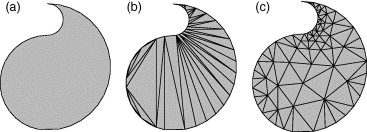
\includegraphics[width=0.55\textwidth]{images/introduction/triangulation.jpg}
		\end{figure}
}
\only<2>
{
	\begin{itemize}
		\item Ejemplo 3D
	\end{itemize}
	\begin{figure}
		\center
			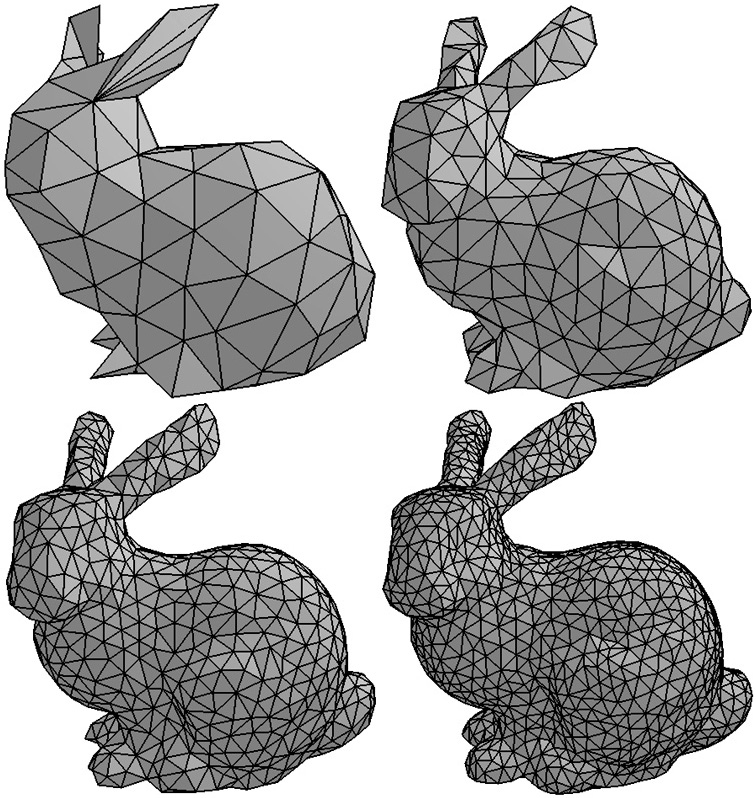
\includegraphics[width=0.5\textwidth]{images/introduction/mesh_remeshing2.jpg}
	\end{figure}
}
\end{frame}

\subsection{Usos de las Mallas Geométricas}

\begin{frame}
\frametitle{Usos de las Mallas Geométricas}
	\begin{block}<1->{Simulaciones físicas}
		\begin{itemize}[<+->]
			\item Estudio de fuerzas.
			\item Interaccion de objetos.
			\item Simulacion de fluidos.
		\end{itemize}
	\end{block}
	\begin{block}<4->{Gráficos}
		\begin{itemize}[<+->]
			\item Visualización de cuerpos en tres dimensiones.
			\item Visualización de funciones matemáticas.
		\end{itemize}
	\end{block}
	\begin{varblock}[0.9\textwidth]{Artísticos}<6->
		\begin{itemize}[<+->]
			\item Gráficos realistas.
			\item Animación.
			\item Películas.
		\end{itemize}
	\end{varblock}
\end{frame}


\subsection{Consideraciones Físicas}
\begin{frame}
	\frametitle{Consideraciones Físicas}
	\begin{itemize}[<+->]
		\item Vivimos en un mundo en tres dimensiones.
			\begin{itemize}
				\item Posición específica dentro de un espacio continuo.
				\item No existe una distancia mínima para el desplazamiento.
			\end{itemize}
		\item La continuidad representa un problema en el mundo virtual.
		\item \emph{Continuous Collision Detection}.
		\item Los objetos estan compuestos de materia.
			\begin{itemize}
				\item Los objetos en el mundo vitual no están (ni pueden aún) ser
							descritos por unidades atómicas.
			\end{itemize}
		\item Los objetos en el mundo virtual son representados por una cantidad discreta
					de triángulos, formando una superficie.
		\item Simples discretizaciones de los objetos reales, sin propiedades físicas como el roce.
			\begin{itemize}
				\item Mesa infinitamente lisa.
			\end{itemize}
	\end{itemize}
\end{frame}

\subsection{Objetos en tres dimensiones}
\begin{frame}
	\frametitle{Objetos en tres dimensiones}
	\begin{itemize}[<+->]
		\item Conjunto de planos triangulares que forman la superficie externa y visible del objeto.
		\item Para extraer la información de la forma de un objeto existen diversas tecnologías.
			\begin{itemize}
				\item Software capaz de generar modelos usando arreglo de fotografías.
				\item Arreglo de cámaras que capturan en tiempo real una nube de puntos infrarrojos.
				\item Equipos de imagenología de resonancia magnética.
					\begin{itemize}
						\item Técnica no invasiva que utiliza el fenómeno de la resonancia magnética, obtiene
									información de la estructura y composición del cuerpo a analizar.
						\item La información obtenida procesada por un software que genera una malla
									geométrica del área de interés
						\item ;)
					\end{itemize}
			\end{itemize}
	\end{itemize}
\end{frame}

\subsection{Objetivos}
\begin{frame}
	\frametitle{Objetivos}
	\begin{itemize}[<+->]
		\item Se propondrá un flujo de trabajo que permita la extracción de una superficie
					dada una colección de puntos en un espacio tridimensional.
			\begin{itemize}
				\item Se hará énfasis en los primeros pasos del flujo propuesto.
			\end{itemize}
		\item Para ello se estudiará el algoritmo de \emph{Marching Cubes}.
			\begin{itemize}
				\item Hacer la extracción de una malla de superficie.
			\end{itemize}
		\item Se construirá una herramienta de visualización y navegación que ayudará a la correcta
					elección del valor mínimo para poder extraer una superficie con un nivel de detalle controlable por el investigador.
	\end{itemize}
\end{frame}

\section{Estado del Arte}
\subsection{Marching Squares}

\begin{frame}
	\frametitle{Marching Squares}

		\only<2>
		{
			\begin{figure}[h]
				\centering
					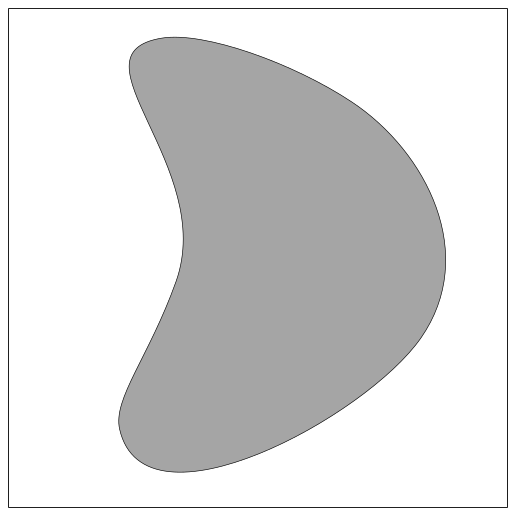
\includegraphics[width=0.5\textwidth]{../images/marchingsquare/marchingsquares_1.pdf}
			\end{figure}
		}
		\only<3>
		{
			\begin{figure}[h]
				\centering
					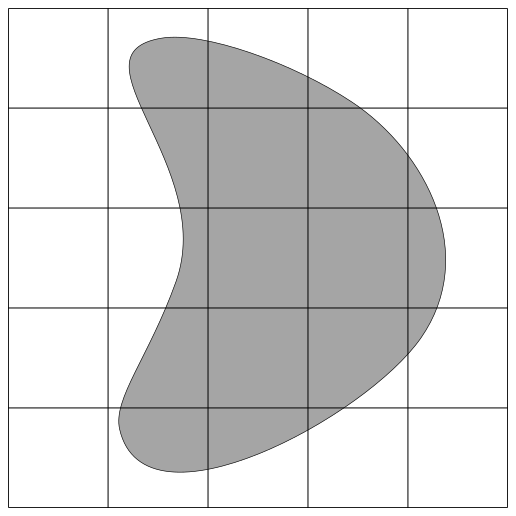
\includegraphics[width=0.5\textwidth]{../images/marchingsquare/marchingsquares_2.pdf}
			\end{figure}
		}
		\only<4>
		{
			\begin{figure}[h]
				\centering
					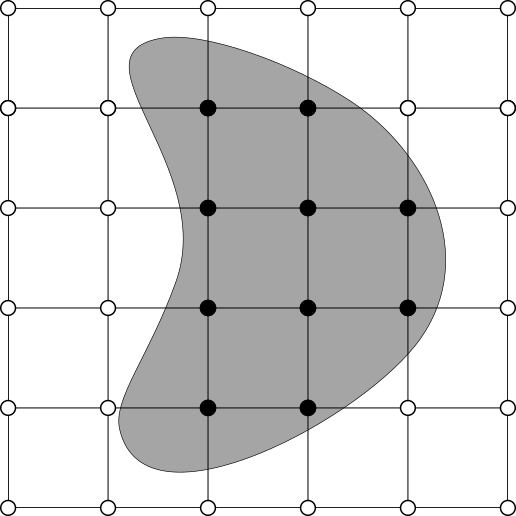
\includegraphics[width=0.5\textwidth]{../images/marchingsquare/marchingsquares_3.pdf}
			\end{figure}
		}
		\only<5>
		{
			\begin{figure}[h]
				\centering
					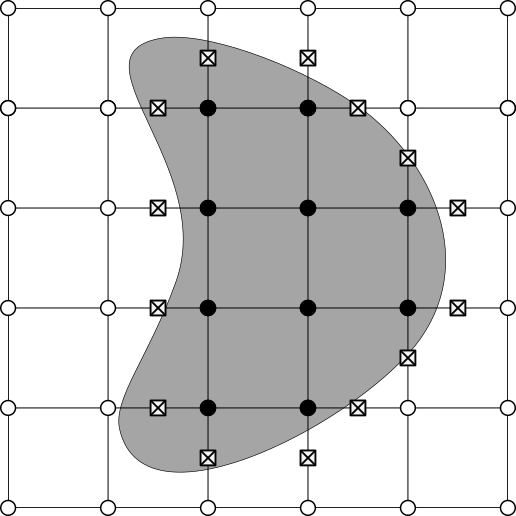
\includegraphics[width=0.5\textwidth]{../images/marchingsquare/marchingsquares_4.pdf}
			\end{figure}
		}
		\only<6>
		{
			\begin{figure}[h]
				\centering
					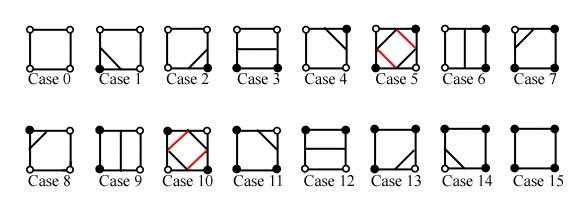
\includegraphics[width=1.0\textwidth]{../images/marchingsquare/cases.png}
			\end{figure}
		}
		\only<7>
		{
			\begin{figure}[h]
				\centering
					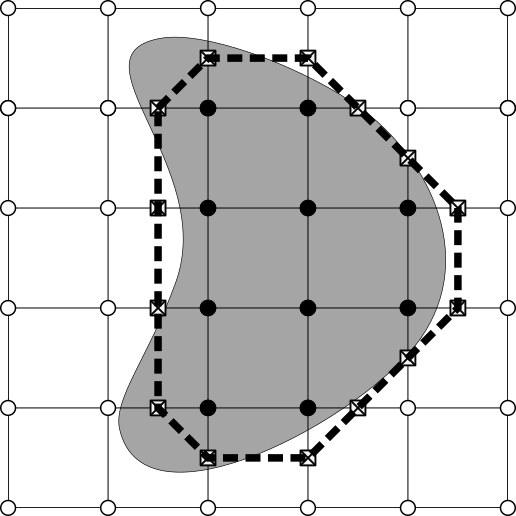
\includegraphics[width=0.5\textwidth]{../images/marchingsquare/marchingsquares_5.pdf}
			\end{figure}
		}
		\only<8>
		{
			\begin{figure}[h]
				\centering
					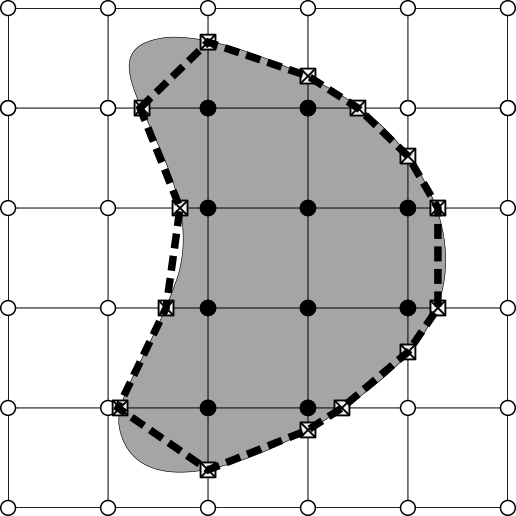
\includegraphics[width=0.5\textwidth]{../images/marchingsquare/marchingsquares_6.pdf}
			\end{figure}
		}
\end{frame}

%\subsubsection{Discusión}

\begin{frame}
	\frametitle{Discusión}
	\begin{columns}[onlytextwidth]

		\begin{column}{0.45\textwidth}<2->

			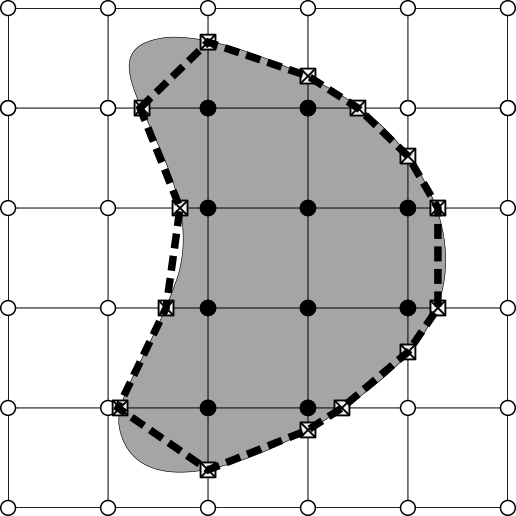
\includegraphics[width=\textwidth]{../images/marchingsquare/marchingsquares_6.pdf}

		\end{column}

		\begin{column}{0.45\textwidth}<2->

			\begin{varblock}[\textwidth]{}
				\begin{enumerate}
					\item<3-> Contorno obtenido no es preciso
					\item<4-> Solución directa
						\begin{enumerate}
							\item<5-> Aumentar divisiones
						\end{enumerate}
					\item<6-> Otras Técnicas
						\begin{enumerate}
							\item<7-> Técnicas Adaptativas
						\end{enumerate}
				\end{enumerate}
			\end{varblock}

		\end{column}

	\end{columns}
\end{frame}

\begin{frame}
	\frametitle{Discusión}
	\begin{columns}[onlytextwidth]

		\begin{column}{0.45\textwidth}<2->

			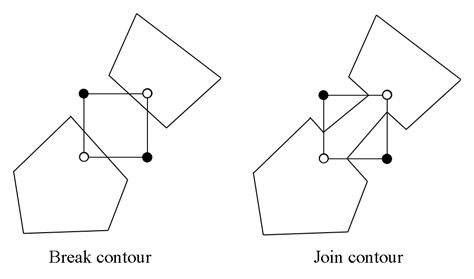
\includegraphics[width=\textwidth]{../images/marchingsquare/marchingSAmbEx.png}

		\end{column}

		\begin{column}{0.45\textwidth}<2->

			\begin{varblock}[\textwidth]{}
				\begin{enumerate}
					\item<3-> Ambigüedad
						\begin{enumerate}
							\item<4-> Vertices diagonales marcados
						\end{enumerate}
				\end{enumerate}
			\end{varblock}

		\end{column}

	\end{columns}
\end{frame}

\subsection{Marching Cubes}

\begin{frame}
	\frametitle{Marching Cubes}

	\uncover<2->
	{
		\begin{varblock}[\textwidth]{¿Que és?}
			\begin{enumerate}
				\item<3-> Marching Cubes es un algoritmo de extracción de una superficie poligonal de un cuerpo en un espacio escalar en tres dimensiones.
				\item<4-> Idea.
					\begin{enumerate}
						\item<5-> Forma $\rightarrow$ Cuerpo.
						\item<6-> Cuadrados $\rightarrow$ Cubos.
					\end{enumerate}
			\end{enumerate}
		\end{varblock}
	}
	\uncover<7->
	{
		\begin{varblock}[\textwidth]{Aplicaciones}
			\begin{enumerate}
				\item<8-> Reconstrucción de superficies de un dataset de imágenes medicas.
				\item<9-> Contorno tridimensional de una función matemática.
				\item<10-> Video! ;).
			\end{enumerate}
		\end{varblock}
	}
\end{frame}

\begin{frame}
	\frametitle{Marching Cubes}

	\begin{varblock}[\textwidth]{¿Cuántos casos tiene Marching Cubes?}
		\begin{enumerate}
			\item<2-> Un Cubo tiene 6 caras, 8 vértices y 12 aristas.
			\item<3-> Cada vértice puede tener 2 estados.
			\item<4-> 256 combinaciones posibles.
			\item<5-> Pueden ser reducidos.
				\begin{enumerate}
					\item<6-> 2 casos triviales.
					\item<7-> Caso de 1 sólo vértice, hay 8 iguales.
					\item<8-> Simetria\uncover<9->{: 14 casos en los restantes 254.}
				\end{enumerate}
		\end{enumerate}
	\end{varblock}

\end{frame}

\begin{frame}
	\frametitle{Marching Cubes}

	Finalmente\uncover<2->{, las quince familias de casos de Marching Cubes:}

	\uncover<3->
	{
		\begin{figure}[h]
			\centering
				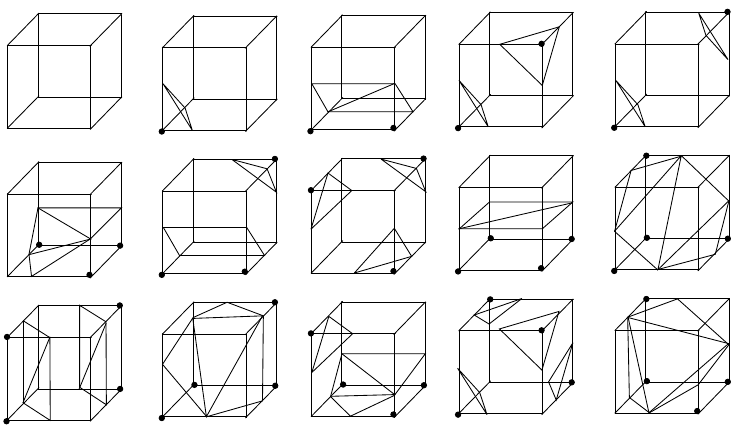
\includegraphics[width=0.8\textwidth]{../images/marchingcubes/Shu95adaptivemarching_1.png}
		\end{figure}
	}
\end{frame}

\begin{frame}
	\frametitle{Procedimiento}

	\only<1>{El procedimiento es el mismo que en Marching Squares, el espacio se divide en un arreglo de regiones cúbicas.}

	\only<2>
	{
		\begin{figure}[h]
			\centering
				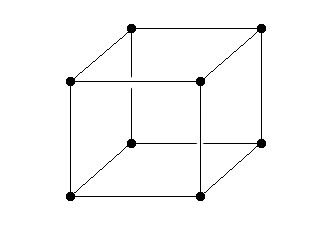
\includegraphics[width=0.7\textwidth]{../images/marchingcubes/cube_01.png}
		\end{figure}
	}
	\only<3>
	{
		\begin{figure}[h]
			\centering
				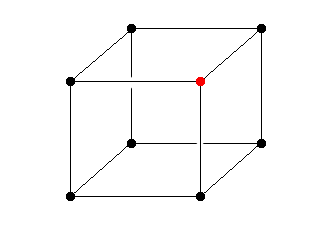
\includegraphics[width=0.7\textwidth]{../images/marchingcubes/cube_02.png}
		\end{figure}
	}
	\only<4>
	{
		\begin{figure}[h]
			\centering
				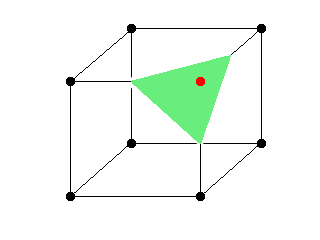
\includegraphics[width=0.7\textwidth]{../images/marchingcubes/cube_03.png}
		\end{figure}
	}
	\only<5>
	{
		Video :)
	}
\end{frame}

\begin{frame}
	\frametitle{Discusión}
	\begin{columns}[onlytextwidth]

		\begin{column}{0.45\textwidth}<2->

			\begin{varblock}[\textwidth]{}
				\begin{enumerate}
					\item<3-> Mismas falencias
						\begin{enumerate}
							\item<4-> Sin interpolación y dependiendo de la resolución.
						\end{enumerate}
					\item<6-> Pero al aumentar la resolución...
						\begin{enumerate}
							\item<10-> Requiere más cómputo.
						\end{enumerate}
				\end{enumerate}
			\end{varblock}

		\end{column}

		\begin{column}{0.45\textwidth}<2->

			\only<5-6>
			{
				\includegraphics[width=\textwidth]{../images/marchingcubes/mc_blobs.png}
			}
			\only<7>
			{
				\includegraphics[width=\textwidth]{../images/marchingcubes/mc_blobs_12.png}
			}
			\only<8>
			{
				\includegraphics[width=\textwidth]{../images/marchingcubes/mc_blobs_20.png}
			}
			\only<9-10>
			{
				\includegraphics[width=\textwidth]{../images/marchingcubes/mc_blobs_50.png}
			}

		\end{column}

	\end{columns}
\end{frame}

\begin{frame}
	\frametitle{Discusión}

	\begin{varblock}[\textwidth]{El principal problema}
		\begin{enumerate}
			\item<2-> Ambigüedad.
				\begin{enumerate}
					\item<4-> Ambigüedades externas.
					\item<5-> Ambigüedades internas.
					\item<6-> 2 poligonizaciones distintas para el mismo caso diagonal.
				\end{enumerate}
		\end{enumerate}
	\end{varblock}

	\only<3>
	{
		\centering
			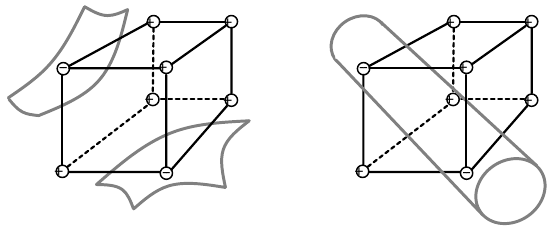
\includegraphics[width=0.7\textwidth]{../images/marchingcubes/Bloomenthal88polygonizationof_1.png}
	}
	\only<4>
	{
		\centering
			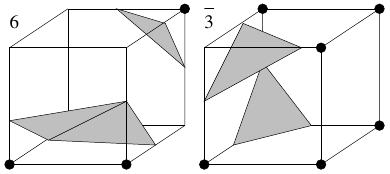
\includegraphics[width=0.7\textwidth]{../images/marchingcubes/Chernyaev95marchingcubes_1.png}
	}
	\only<5>
	{
		\centering
			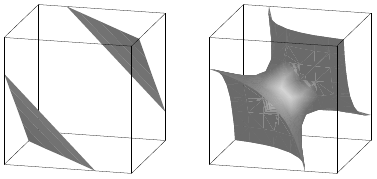
\includegraphics[width=0.7\textwidth]{../images/marchingcubes/Chernyaev95marchingcubes_2.png}
	}
	\only<6>
	{
		\centering
			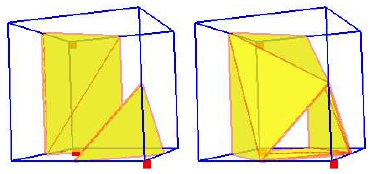
\includegraphics[width=0.7\textwidth]{../images/marchingcubes/Lewiner03efficientimplementation_2.png}
	}

\end{frame}

\begin{frame}
	\frametitle{Discusión}

	\begin{varblock}[\textwidth]{Formas de evitar estos problemas}
		\begin{enumerate}
			\item<2-> Usando otras subdivisiones.
			\item<3-> Tetraedros, es la descomposición lineal más simple en tres dimensiones.
			\item<4-> Cinco divisiones tetraédricas.
			\item<5-> Doce divisiones tetraédricas.
		\end{enumerate}
	\end{varblock}

	\only<4>
	{
		\centering
			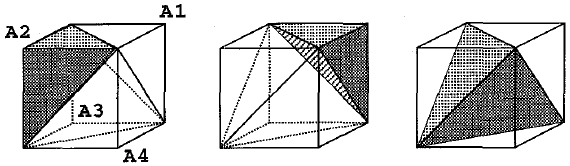
\includegraphics[width=0.7\textwidth]{../images/marchingcubes/GueziecHummel95exploitingtriangulated_1.png}
	}
	\only<5>
	{
		\centering
			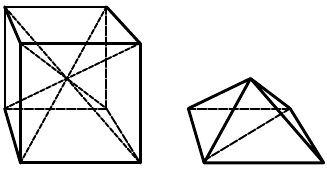
\includegraphics[width=0.5\textwidth]{../images/marchingcubes/Bloomenthal88polygonizationof_2.png}
	}

\end{frame}

\section{Propuesta}
\subsection{Flujo de Trabajo}

\begin{frame}
	\frametitle{Flujo de Trabajo}

	\begin{figure}
		\centering
			\includegraphics[width=0.45\textwidth]{../images/misc/workflow.pdf}
	\end{figure}
\end{frame}

\begin{frame}
	\frametitle{Flujo de Trabajo}

	\begin{varblock}[\textwidth]{Extracción de Datos}
		\begin{enumerate}
			\item<2-> Para extraer una superficie de una nube de puntos es necesario recolectar esos puntos.
			\item<3-> Existen diversas técnicas, pero para el propósito de este trabajo, se utilizarán \emph{datasets}.
				\begin{enumerate}
					\item<4-> Imágenes por resonancia magnética.
					\item<5-> Funciones en tres dimensiones.
				\end{enumerate}
		\end{enumerate}
	\end{varblock}
\end{frame}

\begin{frame}
	\frametitle{Flujo de Trabajo}

	Imágenes por resonancia magnética

	\begin{figure}
		\centering
			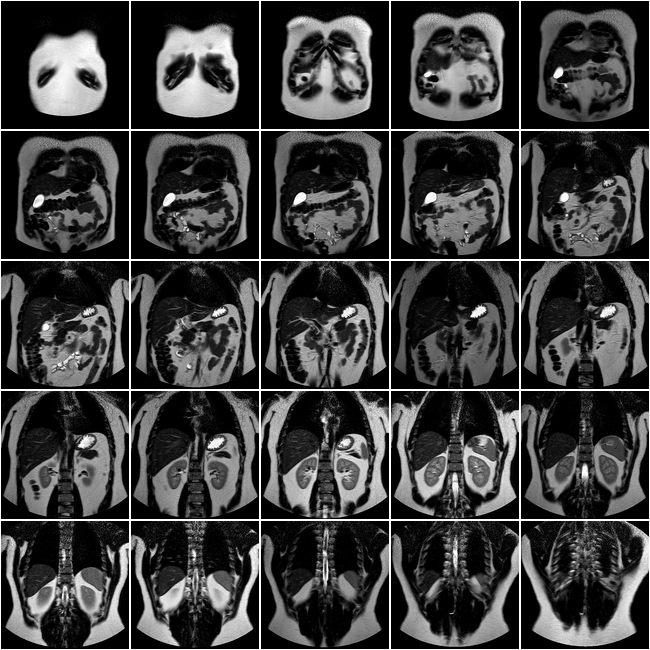
\includegraphics[width=0.55\textwidth]{../images/misc/mri_joe.png}
	\end{figure}
\end{frame}

\begin{frame}
	\frametitle{Flujo de Trabajo}

	Funciones en tres dimensiones

	\begin{figure}
		\centering
			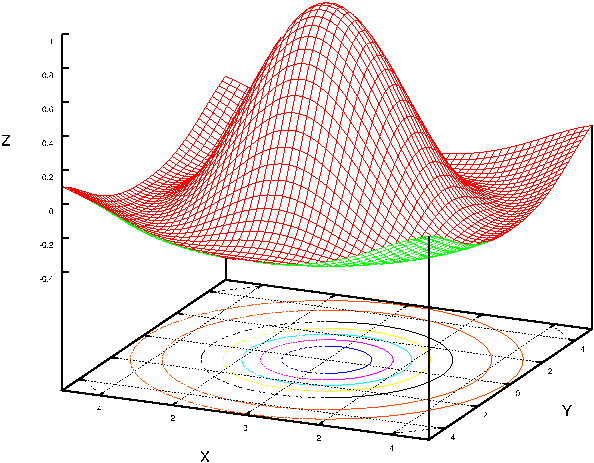
\includegraphics[width=0.7\textwidth]{../images/misc/contour_1_using_eps2eps.pdf}
	\end{figure}
\end{frame}

\begin{frame}
	\frametitle{Flujo de Trabajo}

	Funciones en tres dimensiones

	\begin{figure}
		\centering
			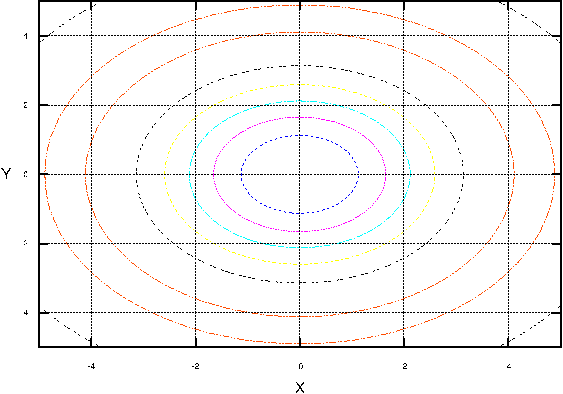
\includegraphics[width=0.7\textwidth]{../images/misc/contour_2_using_eps2eps.pdf}
	\end{figure}
\end{frame}

\begin{frame}
	\frametitle{Flujo de Trabajo}

	\begin{varblock}[\textwidth]{Conversión de imágenes}
		\begin{enumerate}
			\item<2-> Debido a las distintas posibles fuentes de datos, las imágenes estarán en distintos formatos.
			\item<3-> Garantizar independencia de esto.
			\item<4-> Unificación.
			\item<5-> Un formato común.
			\item<6-> PGM \emph{Portable GreyMap}.
		\end{enumerate}
	\end{varblock}
\end{frame}

\begin{frame}
	\frametitle{Flujo de Trabajo}

	\begin{varblock}[\textwidth]{Selección del Isovalor}
		\begin{enumerate}
			\item<2-> Es una constante que define qué pixeles estarán dentro o fuera.
			\item<3-> Ejemplo de iluminación.
			\item<4-> Ambito médico, no es trivial.
				\begin{enumerate}
					\item<5-> Puede marcar diferencia entre ver al nivel de la piel, o nivel de los huesos.
				\end{enumerate}
			\item<6-> Escala porcentual.
		\end{enumerate}
	\end{varblock}
\end{frame}

\begin{frame}
	\frametitle{Flujo de Trabajo}

	Distintos isovalores

	\only<2>
	{
		\begin{figure}
			\centering
			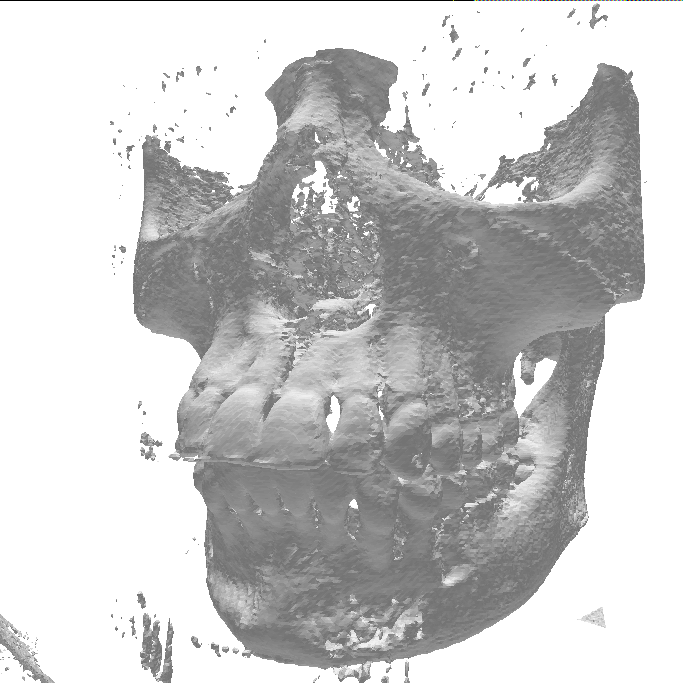
\includegraphics[width=0.5\textwidth]{../images/flujo/isovalue/screenshot_15.png}
			\caption{isovalor: 15\%}
		\end{figure}
	}
	\only<3>
	{
		\begin{figure}
			\centering
			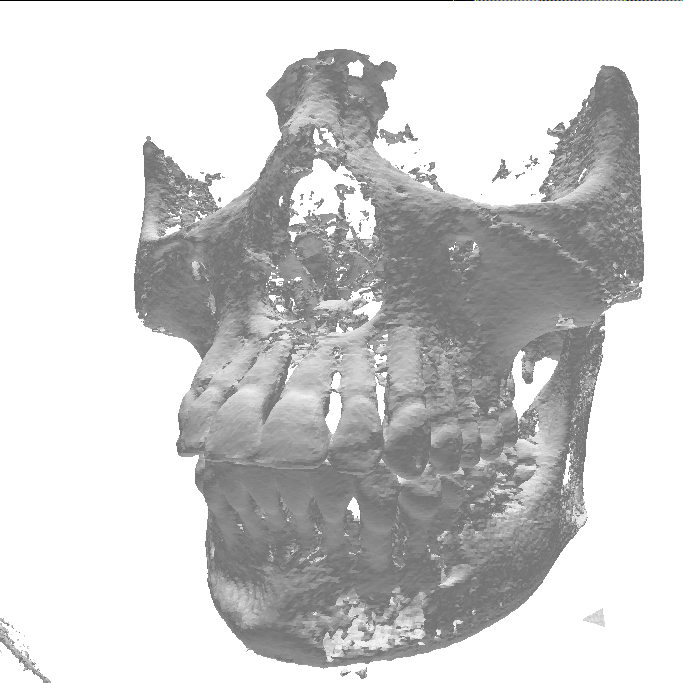
\includegraphics[width=0.5\textwidth]{../images/flujo/isovalue/screenshot_20.png}
			\caption{isovalor: 20\%}
		\end{figure}
	}
	\only<4>
	{
		\begin{figure}
			\centering
			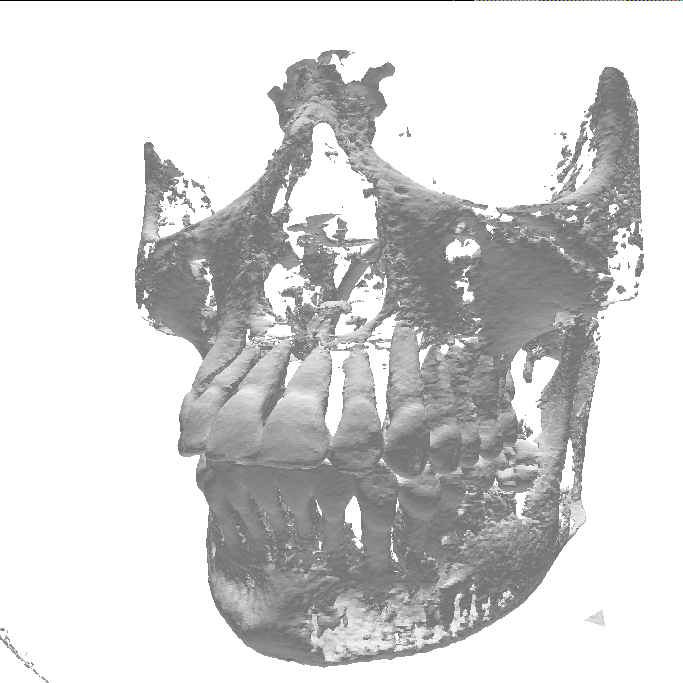
\includegraphics[width=0.5\textwidth]{../images/flujo/isovalue/screenshot_25.png}
			\caption{isovalor: 25\%}
		\end{figure}
	}
	\only<5>
	{
		\begin{figure}
			\centering
			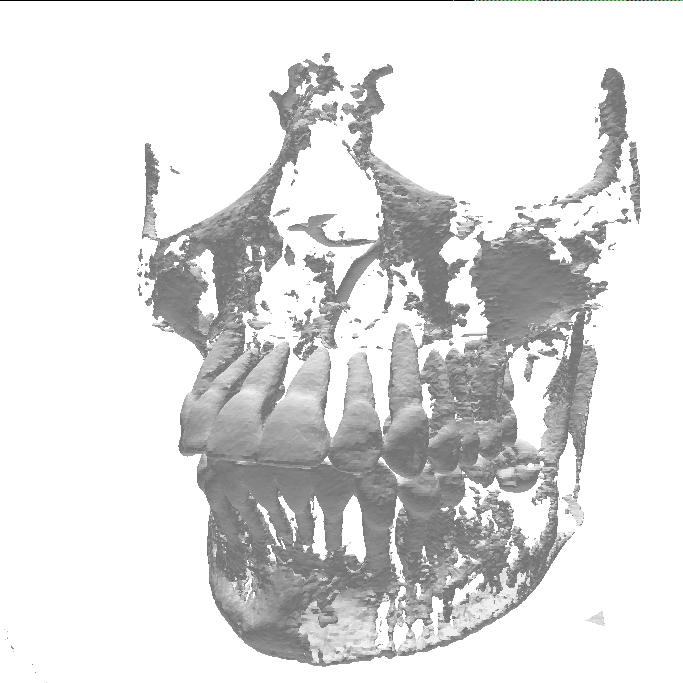
\includegraphics[width=0.5\textwidth]{../images/flujo/isovalue/screenshot_30.png}
			\caption{isovalor: 30\%}
		\end{figure}
	}
	\only<6>
	{
		\begin{figure}
			\centering
			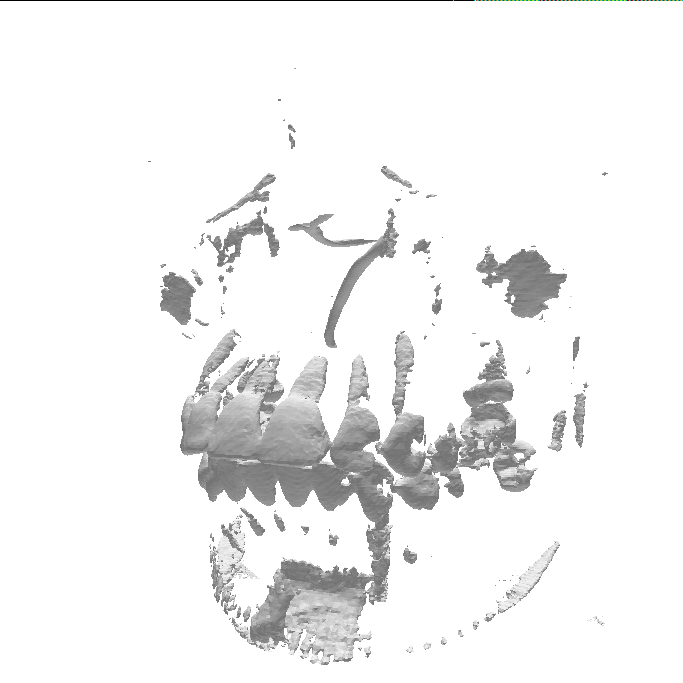
\includegraphics[width=0.5\textwidth]{../images/flujo/isovalue/screenshot_40.png}
			\caption{isovalor: 40\%}
		\end{figure}
	}
	\only<7>
	{
		\begin{figure}
			\centering
			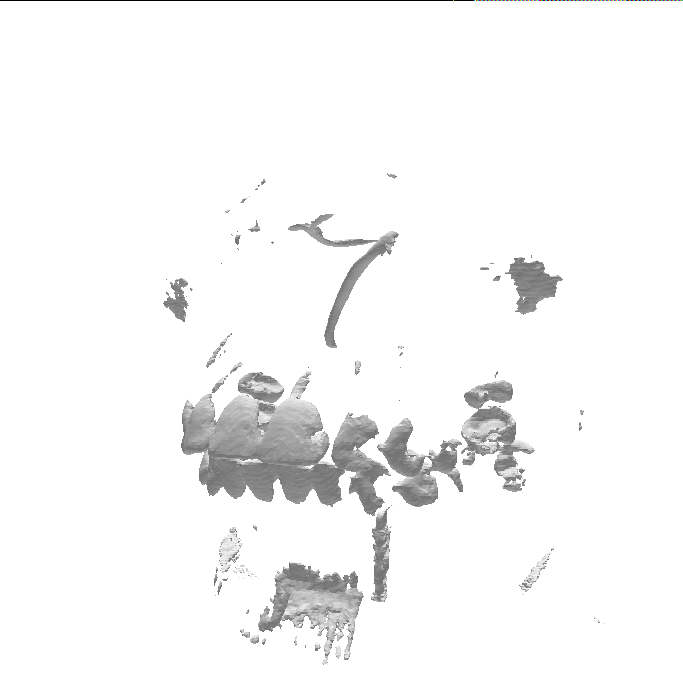
\includegraphics[width=0.5\textwidth]{../images/flujo/isovalue/screenshot_45.png}
			\caption{isovalor: 45\%}
		\end{figure}
	}
	\only<8>
	{
		\begin{figure}
			\centering
			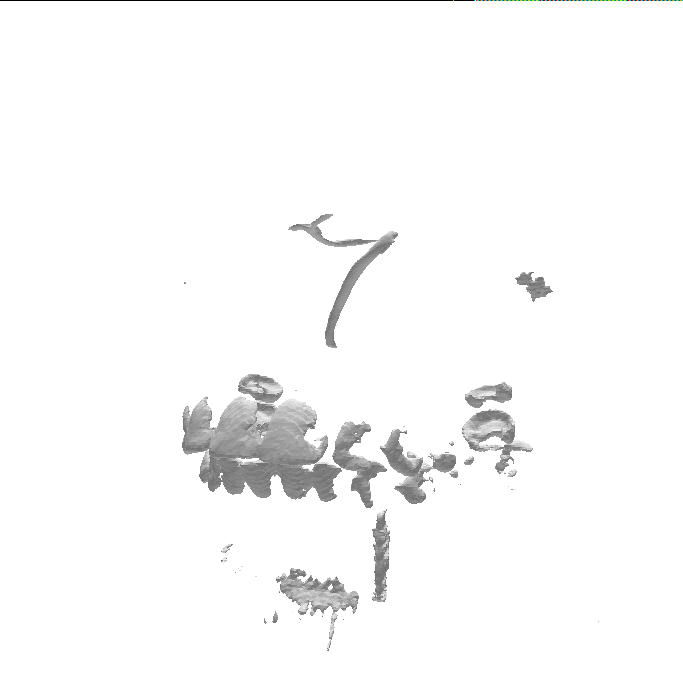
\includegraphics[width=0.5\textwidth]{../images/flujo/isovalue/screenshot_50.png}
			\caption{isovalor: 50\%}
		\end{figure}
	}
	\only<9>
	{
		\begin{figure}
			\centering
			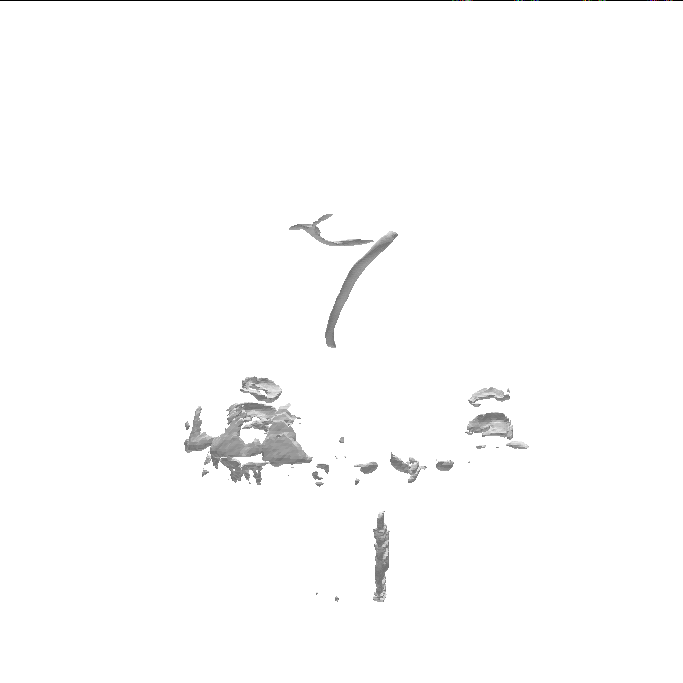
\includegraphics[width=0.5\textwidth]{../images/flujo/isovalue/screenshot_60.png}
			\caption{isovalor: 60\%}
		\end{figure}
	}
	\only<10>
	{
		\begin{figure}
			\centering
			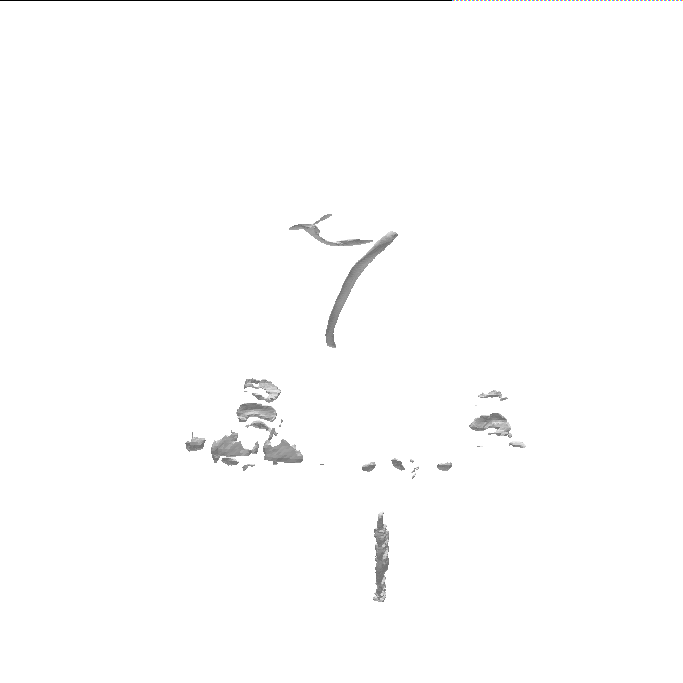
\includegraphics[width=0.5\textwidth]{../images/flujo/isovalue/screenshot_65.png}
			\caption{isovalor: 65\%}
		\end{figure}
	}
	\only<11>
	{
		\begin{figure}
			\centering
			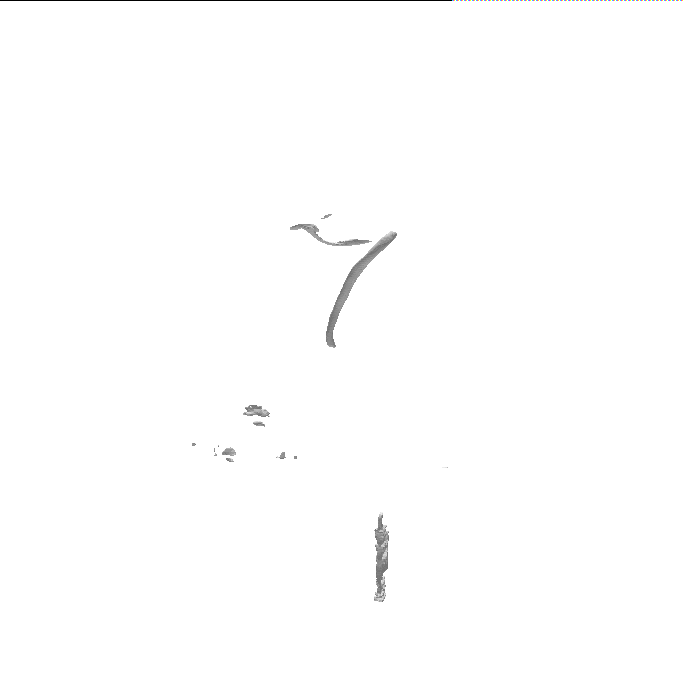
\includegraphics[width=0.5\textwidth]{../images/flujo/isovalue/screenshot_75.png}
			\caption{isovalor: 75\%}
		\end{figure}
	}
	\only<12>
	{
		\begin{figure}
			\centering
			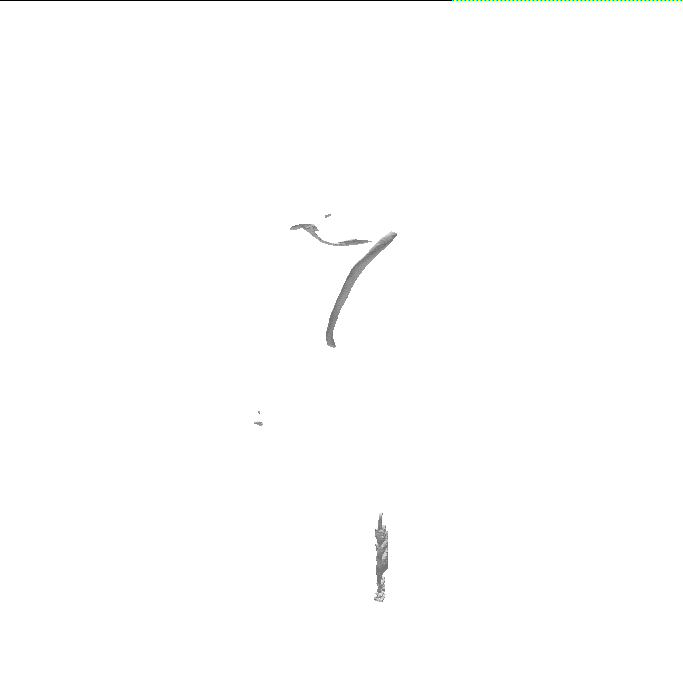
\includegraphics[width=0.5\textwidth]{../images/flujo/isovalue/screenshot_80.png}
			\caption{isovalor: 80\%}
		\end{figure}
	}
	\only<13>
	{
		\begin{figure}
			\centering
			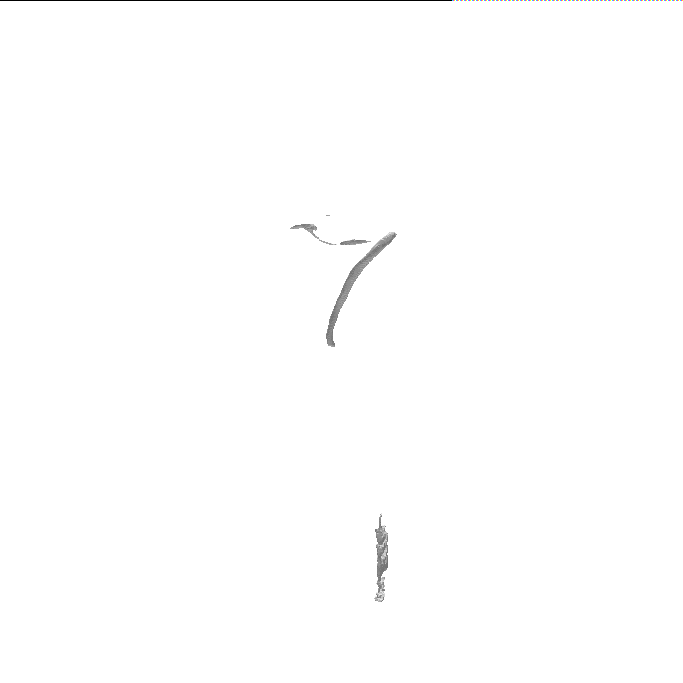
\includegraphics[width=0.5\textwidth]{../images/flujo/isovalue/screenshot_90.png}
			\caption{isovalor: 90\%}
		\end{figure}
	}
\end{frame}

\begin{frame}
	\frametitle{Flujo de Trabajo}

	\begin{varblock}[\textwidth]{Extracción de la superficie}
		\begin{enumerate}
			\item<2-> Luego de escoger el isovalor adecuado, se procede a extraer una superficie.
			\item<3-> Isosuperficie.
		\end{enumerate}
	\end{varblock}
\end{frame}

\begin{frame}
	\frametitle{Flujo de Trabajo}

	\begin{varblock}[\textwidth]{Extracción de la superficie}
		\begin{enumerate}[<+->]
			\item Este trabajo tiene su mayor enfoque en esta parte.
				\begin{enumerate}[<+->]
					\item Se hizo un programa que implementa Marching Cubes, y genera una superficie usando un isovalor ajustable.
					\item Permite visualizar y navegar en tres dimensiones el modelo generado.
					\item Permite modificar el isovalor en tiempo real, y volver a generar el modelo, mientras se navega.
					\item Permite sacar capturas de pantalla, y exportación de los modelos generados a un archivo de modelos 3D estándar y abierto: \emph{OFF}.
				\end{enumerate}
		\end{enumerate}
	\end{varblock}
\end{frame}

\begin{frame}
	\frametitle{Flujo de Trabajo}

	LLego el momento!

	\only<2>
	{
		\begin{figure}
			\centering
				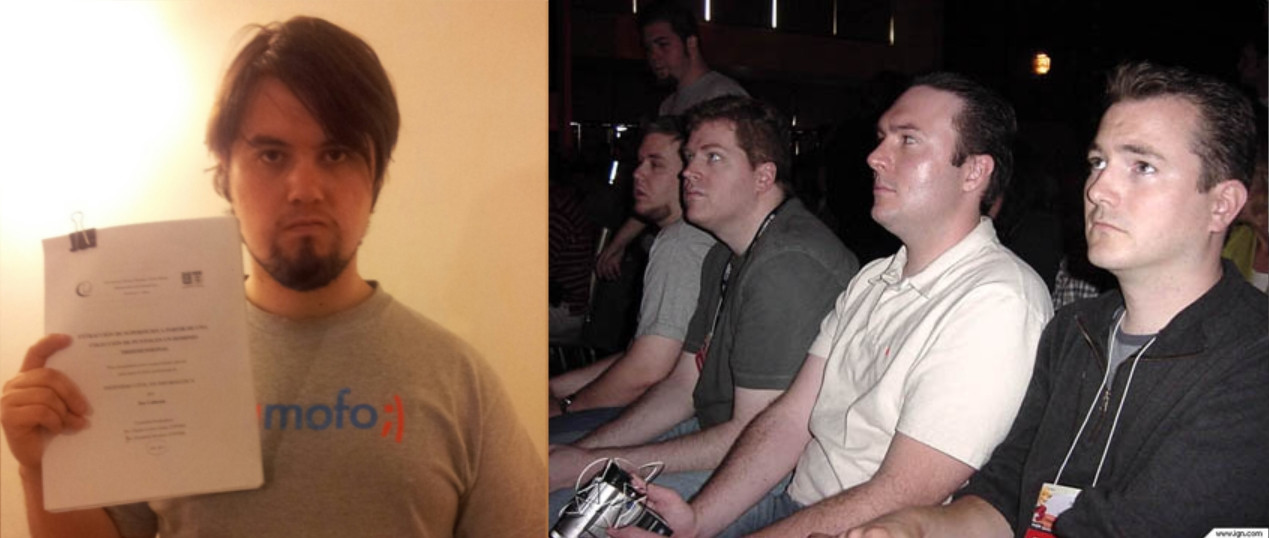
\includegraphics[width=1.0\textwidth]{images/joe0.jpg}
		\end{figure}
	}
	\only<3>
	{
		\begin{figure}
			\centering
				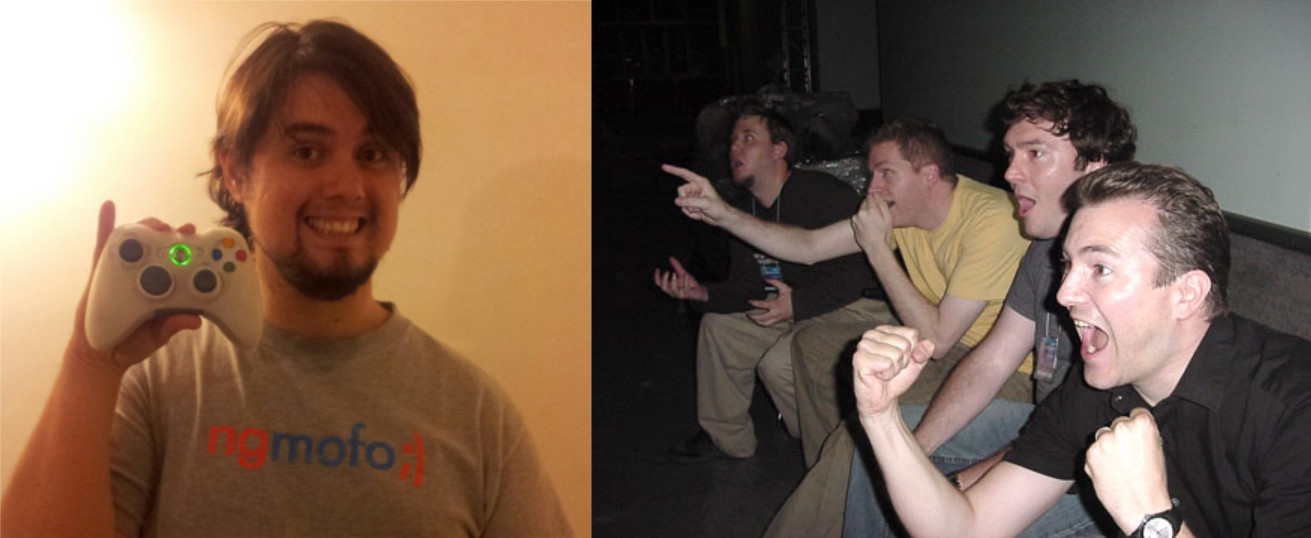
\includegraphics[width=1.0\textwidth]{images/joe1.jpg}
		\end{figure}
	}

\end{frame}

\begin{frame}
	\frametitle{Flujo de Trabajo}

	\begin{varblock}[\textwidth]{Refinamiento}
		\begin{enumerate}
			\item<2-> Luego de extraer la isosuperficie, es momento de refinar con el fin de mejorar su calidad, en los términos que se estimen convenientes pasa cada propósito.
				\begin{enumerate}
					\item<3-> Cantidad de triángulos.
					\item<4-> Aliasing.
					\item<5-> Topología.
				\end{enumerate}
		\end{enumerate}
	\end{varblock}

\end{frame}

\begin{frame}
	\frametitle{Flujo de Trabajo}

	\begin{varblock}[\textwidth]{Refinamiento}
		\begin{enumerate}
			\item<2-> CGAL.
				\begin{enumerate}
					\item<3-> \emph{The Computational Geometry Algorithms Library}.
					\item<4-> C++.
					\item<5-> Acceso fácil y eficiente a una colección de algoritmos geométricos.
				\end{enumerate}
					\begin{enumerate}
						\item<6-> Triangulaciones.
						\item<7-> Generación de mallas.
						\item<8-> Procesamiento geométrico (esto se busca).
					\end{enumerate}
				\item<9-> Toma una colección de puntos con sus normales orientadas, y genera una superficie calculando una funcion implícita.
		\end{enumerate}
	\end{varblock}

\end{frame}

\begin{frame}
	\frametitle{Flujo de Trabajo}

	\only<1>
	{
		\begin{figure}
			\centering
				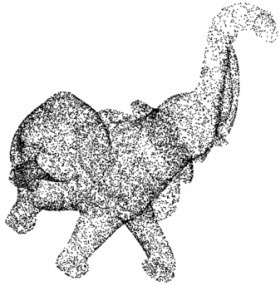
\includegraphics[width=0.5\textwidth]{../images/flujo/refinamiento_1_0.jpg}
		\end{figure}
	}
	\only<2>
	{
		\begin{figure}
			\centering
				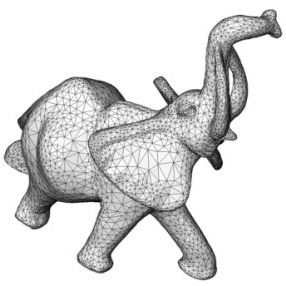
\includegraphics[width=0.5\textwidth]{../images/flujo/refinamiento_1_1.jpg}
		\end{figure}
	}
\end{frame}

\begin{frame}
	\frametitle{Flujo de Trabajo}

	\begin{varblock}[\textwidth]{Exportación}
		\begin{enumerate}
			\item<2-> Hasta este punto ya se tiene la isosuperficie buscada.
				\begin{enumerate}
					\item<2-> Extracción.
					\item<2-> Selección del isovalor.
					\item<2-> Extracción de superficie.
					\item<2-> Refinamiento.
				\end{enumerate}
			\item<2-> El último paso, es exportar al formato útil para el proósito.
		\end{enumerate}
	\end{varblock}

\end{frame}

\section{Conclusiones}

\begin{frame}
	\frametitle{Conclusiones}

	\begin{varblock}[\textwidth]{En general}
		\begin{enumerate}
			\item<2-> Mallas geométricas, son una gran herramienta en la ciencia e ingienería.
			\item<3-> Implicaciones físicas: no se puede hacer un estudio infinitesimal.
		\end{enumerate}
	\end{varblock}

\end{frame}

\begin{frame}
	\frametitle{Conclusiones}

	\begin{varblock}[\textwidth]{Para fines de visualización}
		\begin{enumerate}
			\item<2-> Existen divesas técnicas basadas en elementos finitos.
				\begin{enumerate}
					\item<3-> Marching Squares.
					\item<4-> Marching Cubes.
					\item<5-> Marching Tetrahedrons.
				\end{enumerate}
			\item<6-> Pero tienen sus debilidades.
				\begin{enumerate}
					\item<7-> Malas aproximaciones.
					\item<8-> Mejorarlas requieren un mayor poder de cómputo.
					\item<9-> Problemas topológicos, errores de calculo importantes.
				\end{enumerate}
		\end{enumerate}
	\end{varblock}

\end{frame}

\begin{frame}
	\frametitle{Conclusiones}

	\begin{varblock}[\textwidth]{Objetivos}
		\begin{enumerate}
			\item<2-> Se cumplen los objetivos de estre trabajo.
				\begin{itemize}
					\item<3-> Se propuso un flujo de trabajo que permite la extracción de una superficie
					desde la recolección de los datos (nube de puntos) hasta el modelo final.
					\item<4-> Se mostró la importancia de tomar buenas decisiones en los primeros pasos del flujo, además se facilitó el proceso de selección de un isovalor adecuado.
					\item<5-> Se estudió y se implementó el algoritmo de Marching Cubes.
					\item<6-> Extrae una superficie.
					\item<7-> Y con ello se construyó una herramienta de visualización y navegación que ayudará a la correcta elección del isovalor para poder extraer una superficie con un nivel de detalle controlable por el investigador.
				\end{itemize}
		\end{enumerate}
	\end{varblock}

\end{frame}

\section{Trabajo a Futuro}

\begin{frame}
	\frametitle{Trabajo a Futuro}

	\begin{varblock}[\textwidth]{}
		\begin{enumerate}
			\item<2-> Se propuso un flujo de trabajo y se hizo especial énfasis en el paso de extracción de la superficie.
			\item<3-> Este proceso puede ser mejorado.
				\begin{itemize}
					\item<4-> La posición de los vértices obtenidos es calculada usando una interpolación lineal.
					\item<5-> Escala porcentual del isovalor.
					\item<6-> Paralelismo.
					\item<7-> Resolución fija, métodos adaptativos.
					\item<8-> Se implementó el algoritmo de Marching Cubes propuesto por Lorensen y Cline, se pueden ocupar versiones mejoradas.
				\end{itemize}
		\end{enumerate}
	\end{varblock}

\end{frame}

\section*{End}

\begin{frame}
	\frametitle{EOF}
\end{frame}

\begin{frame}
	\frametitle{¿Preguntas?}
\end{frame}

\end{document}
